\documentclass{article}

\usepackage{amsmath}
\usepackage{amssymb}
\usepackage{graphicx}
\graphicspath{{images/}}

\title{The Restricted Three-Body Problem}
\author{Armando Herrera}

\begin{document}
\maketitle

Here I strive to describe the mechanics of the three-body problem. In order to go over the three-body problem, we must first go over the underlying physics, describe the simpler single body problem, two body problems, the three body problem, and finally the restricted three-body problems.

\section{Classical Mechanics}

With classical mechanics it is possible to describe the motion of most object in the universe. Using it, we can describe the motions of certain object in non-extreme environments. For instance, we can use it to describe the motion of a bicycle, the trajectories of billiard balls, etc... . It's limitation start at speeds approaching light speed, in the quantum realm, or near super-massive objects like a black hole. It is built on top of certain physical concepts, some formulated by Issac Newton.

Objects have certain conserved properties to them, under Classical Mechanics, a constant mass, a relative position in space, and a relative velocity in space. We can say that an objects velocity is the rate of change of the position of said object. So, in terms of a derivative: $$\vec{v}=\dot{\vec{r}}$$ 

Here I denote $\vec{r}$ to be the position of the object and $\vec{v}$ to be the velocity of the object. The $\vec{}$ denotes the fact that they are vectors in euclidean space and $\dot{}$ is equivalent to saying $\frac{d}{dt}$.

Similarly, the acceleration of an object can be defined as the rate of change of velocity of said object or the rate of change of the rate of change of the object's position. $$\vec{a}=\dot{\vec{v}}=\ddot{\vec{r}}$$ 
Here I use $a$ to the acceleration and $\ddot{}$ as the second derivative, $\frac{d^2}{dt^2}$.

Newton's second law of motion describe the relationship between force and acceleration, showing that the net force $F$ applied to an object is equal to the mass $m$ multiplied by the acceleration. $$\vec{F}=m\vec{a}$$

Now, there are categories of forces, Contact Forces and Action-at-a-Distance Forces. The differentiating factor between the two categories is that the Contact Forces, as the name implies, requires two object's contact and Action-at-a-Distance Forces are applied, again as the name implies, at a distance. In the vacuum of space the main force active is the Force of Gravity.

The force of gravity, and most Action-at-a-Distance Forces, exist by the inverse-square law, where it's amount is inversely proportional to the distance from the source of the force, here gravity. $$F\propto \frac{1}{r^2}$$ In 1687 Newton in Newton's Principia postulated what is now called Newton's Law of Universal Gravitation \cite{rohrlich_1999}. $$F_{21}=-G\frac{m_1m_2}{r^2}$$ or in vector notation 
\begin{equation}
\vec{F}_{21}=-G\frac{m_1m_2}{|\vec{r}_{12}|^2}\hat{r}_{12}
\end{equation}
 where $\hat{r}$ is the unit vector of $r$.

Newton's Law of Universal Gravitation gives us the key to the story between objects in the vacuum of space. For instance, if we have $n$ objects, the force on object 1 is $$F_1=\sum_{i=2}^n{G\frac{m_1 m_i}{r_{1i}^2}}$$ and, as we see for the calculation for object 1, the computational complexity for a single object is $O(n)$ and therefore to calculate the force on all $n$ objects the complexity is $O(n^2)$. Using these force along with Newton's second law the velocity and position can then be calculated.
\begin{align}
	\vec{v} &= \vec{v}_0+\vec{a}t\\
	\vec{r} &= \vec{r}_0+\bigg(\frac{\vec{v}+\vec{v}_0}{2}\bigg)t
\end{align}
Now, this is enough information to simulate the restricted 3-body system but it is not enough to calculate initial orbit velocities, orbit characteristics, or most optimal trajectory. In fact for large $n$ relying on this law is practically impossible due to the quadratic complexity. Hence, we can use numerical integration to approximate Newton's laws.

Firstly, a more useful representation is that of potential energy. Gravity is a conservative force, meaning that any work done to move an object that is under the influence of gravity isn't path dependent. $$\nabla\times \vec{F}=\vec{0}$$ 
So the potential energy can be calculated by $$U=-\int_C \vec{F}\cdot d\vec{r}.$$ After plugging in $\vec{F}$ and solving the integral we get the gravitational potential energy.
\begin{equation} \label{eq:gravpotential}
U=-G\frac{m_1m_2}{r}
\end{equation}
Another way to represent this is by the gravitational acceleration. 
\begin{equation}
\vec{a}=\frac{GM}{r^2}\hat{r}
\end{equation}

If an object is in orbit around another object and said orbit i circular then we can set the centrifugal acceleration equal to the acceleration due to gravity, $$\frac{v^2}{r}=\frac{GM}{r^2}$$, then solve for velocity.
\begin{equation}
v=\sqrt{\frac{GM}{r}}
\end{equation}

For a non-circular orbit like Elliptical orbits or Parabolic orbits conic sections can be used. Conic sections care the lines where a plane intersects a two napped cone.

\section{Hamiltonian Mechanics}

As complexity is added to a system, calculations done through Newton's formulations become increasingly complex, like in our restricted three body problem. In Hamiltonian Mechanics there are what are called Hamilton's equations. 
\begin{align}
\frac{d\vec{p}}{dt}&=-\frac{\partial \mathcal{H}}{\partial \vec{r}}\\
\frac{d\vec{r}}{dt}&=\frac{\partial \mathcal{H}}{\partial \vec{p}}
\end{align}
Where the hamiltonian, $\mathcal{H}=T+U$, where $T$ is the kinetic energy and $U$ is the potential energy and $p$ is the momentum.

For the two body problem, we can use Hamiltonian Mechanics to analytically express it. $T$ as the kinetic energy, $T=\frac{1}{2}mv^2$, and $U$ the previously calculated gravitational potential energy, equation \ref{eq:gravpotential}. Therefore the Hamiltonian of the system would be $$\mathcal{H}=\frac{1}{2}m_1 v^2-G\frac{m_1 m_2}{r}.$$ Here I am assuming a body is exceptionally larger than the other, $m_2>>m_1$, like in the instance of a space shuttle and the earth. The hamiltonian can be put in terms of the momentum, $p=mv$. 
$$\mathcal{H}=\frac{p_1^2}{2m_1}-G\frac{m_1 m_2}{r}$$
And the solutions would be
\begin{align*}
\frac{\partial \mathcal{H}}{\partial r}&=G\frac{m_1 m_2}{r^2}=F=-\dot{p}\\
\frac{\partial \mathcal{H}}{\partial p}&=\frac{p_1}{m_1}=v_1=\dot{r}
\end{align*}
Notice how the equation for the force of gravity and the velocity was shown.

Now, the restricted three body system, similar to the three body system, where three bodies exist in the system. They differ in that one of the bodies is massive compared to the other two, $m_1>>m_2$ and $m_1>>m_3$, the mass of the third object is smaller than the other two, $m_2>>m_3$, the reference frame's origin is at the center of the massive object, $m_1$, lettings us make some simplifications. The kinetic energy of both bodies, which is the total kinetic energy of the system, is 
$$T=\frac{1}{2}(m_2\vec{v}_2^2+m_3\vec{v}_3^2)$$ and the sum of the gravitation energies of the two bodies 
$$U=-G\frac{m_1}{|\vec{r}_1|^2}-G\frac{m_2}{|\vec{r}_2-\vec{r_1}|^2}$$
\begin{figure}
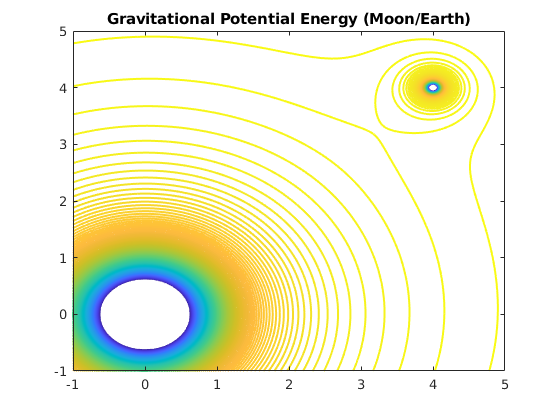
\includegraphics[width=0.85\textwidth]{gravpoten}
\centering
\caption{Plot of the gravitational potential energy between the earth and the moon where distance from the earth and the moon is scaled to 4.}\label{fig:gravpot}
\end{figure}
 Where $r_1$ is the distance from the origin and $r_2$ is the distance from the origin of the second object. A plot of this is shown in Figure~\ref{fig:gravpot}.
Together the hamiltonian is $$\mathcal{H}=\frac{1}{2}(m_2\vec{v}_2^2+m_3\vec{v}_3^2)-G\bigg(\frac{m_1}{|\vec{r}_1|^2}+\frac{m_2}{|\vec{r_2}-\vec{r_1}|^2}\bigg)$$
and if we figure out the momentum of both objects
$$\mathcal{H}=\frac{1}{2}\bigg(\frac{\vec{p}_2^2}{m_2}+\frac{\vec{p}_3^2}{m_3}\bigg)-G\bigg(\frac{m_1}{|\vec{r}_1|^2}+\frac{m_2}{|\vec{r_2}-\vec{r_1}|^2}\bigg).$$ In this case, we can set $r_2$ as constant and evaluate the partial derivative.
\begin{align*}
\dot{p}_3&=G\frac{\partial}{\partial \vec{r}}\bigg(\frac{m_1}{|\vec{r}_1|^2}+\frac{m_2}{|\vec{r_2}-\vec{r_1}|^2}\bigg)\\
\dot{p}_3&=G\bigg(\frac{2m_1}{|\vec{r}_1|^3}+\bigg)\\
\dot{r}_3&=\frac{1}{2}\frac{\partial}{\partial \vec{p}}\bigg(\frac{\vec{p}_2^2}{m_2}+\frac{\vec{p}_3^2}{m_3}\bigg)
\end{align*}

\end{document}